\documentclass[10pt]{article}
\usepackage[utf8]{inputenc}
\usepackage{fontspec}
\usepackage{tabularx}
\usepackage{bbding}
\setmainfont[
    Path = ./,
    Ligatures = TeX,
    BoldFont = SABONLTSTD-BOLD.OTF,
    ItalicFont = SABONLTSTD-ITALIC.OTF,
]{SABONLTSTD-ROMAN.OTF}
\usepackage{book-of-common-prayer}
\geometry{
  paperheight=8.5in,
  paperwidth=5.5in,
  heightrounded,
}

%% TODO: standardize size of music

%% TODO: add a cover image <3
\title{An Order for\\COMPLINE}
\author{}

\begin{document}

\maketitle
\newpage

\section*{Compline}

\instruct{All standing up, the Minister shall say:}

\begin{tabularx}{\linewidth}{lX}
    & The Lord Almighty grant us a quiet night and a perfect end.\\
    \textit{All} & \textbf{Amen.} \\
    \textit{Minister} & O God, make speed to save us; \\
    \textit{All} & \CrossMaltese~\textbf{O Lord, make haste to help us.} \\
\end{tabularx}

\instruct{Then, with all making a profound bow, which is measured by placing
one's hands on one's knees; and rising after the Minister says, ``... The Holy
Ghost'':}

\begin{tabularx}{\linewidth}{lX}
\textit{Minister} & Glory be to the Father, and to the Son, and to the Holy
Ghost; \\
\textit{All} & \textbf{As it was in the beginning, is now, and ever shall
be, world without end. Amen.} \\
     \textit{Minister} & Praise ye the Lord; \\
     \textit{All} & \textbf{The Lord's Name be praised.}
\end{tabularx}

\section*{The Psalms}

\instruct{Then shall be sung or said one  or more of the following Psalms, or
any other suitable Psalms.}

\subsection*{\textbf{Psalm 4}\quad Cum invocarem}

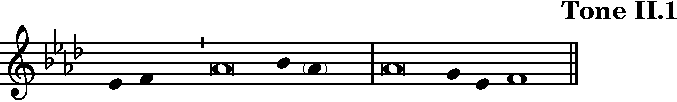
\includegraphics[width=\linewidth]{./psalms/psalm4-crop.pdf}

\begin{enumerate}[
    leftmargin=*,
    label=\textsc { \arabic * }
]
    \item \psalmverse{ {\textsc Hear me} when I call, O God of my \textbf{righ}-teous-ness: }
        {thou hast set me at liberty when I was in trouble; have mercy upon me, and hearken un-\textbf{to} my prayer.}

    \item \psalmverse{O ye sons of men, how long will ye blaspheme min \textbf{hon}-our:}
        {and have such pleasure in vanity, and seek af-\textbf{ter} false-hood?}

    \item \psalmverse{Know this also, that the Lord hath chosen to himself the man that is \textbf{god}-ly:}
        {when I call upon the Lord, he \textbf{will} hear me.}

    \item \psalmverse{Stand in awe, and \textbf{sin} not:}
        {commune with your own heart, and in your cham-\textbf{ber}, and be still.}

    \item \psalmverse{Offer the sacrifice of \textbf{righ}-teous-ness:}
        {and put your trust \textbf{in} the Lord.}

    \item \psalmverse{There be many that say, `Who will show us any \textbf{good}?':}
        {Lord, lift thou up the light of thy countenance \textbf{up}-on us.}

    \item \psalmverse{Thou hast put gladness in my \textbf{heart}:}
        {more than men have when their grain \textbf{wine} in-crease.}

    \item \psalmverse{I will lay me down in peace, and take my \textbf{rest}:}
        {for it is thou, Lord, only, that makest me dwell \textbf{in} safe-ty.}

    \item[] \psalmverse{Glory be to the Father, and to the \textbf{Son}:}
        {and to \textbf{the} Ho-ly Ghost;}

    \item[] \psalmverse{As it was in the beginning, is now, and ever \textbf{shall} be:}
        {world without \textbf{end}. A-men.}
\end{enumerate}

\subsection*{Psalm 31:1-6\quad In te, Domine, speravi}

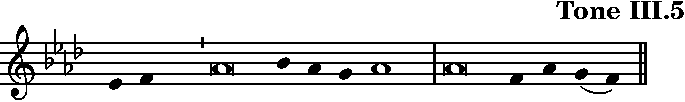
\includegraphics[width=\linewidth]{./psalms/psalm31-crop.pdf}

\begin{enumerate}[
    leftmargin=*,
    label=\textsc { \arabic *}
]

    \item \psalmverse{\textsc{In thee}, O Lord, \textbf{have} I put my trust:}
        {let me never be put to confusion, deliever me in \textbf{thy} righ-teous-nëss.}

    \item \psalmverse{Bow \textbf{down} thine ear to me:}
        {make haste to \textbf{de}-liv-er më.}

    \item \psalmverse{And be thou my strong rock, and \textbf{house} of de-fence:}
        {that thou may-\textbf{est} save më.}

    \item \psalmverse{For thou art my strong rock, \textbf{and} my cas-tle:}
        {be thou also my guide, and lead me for \textbf{thy} Name's säke.}

    \item \psalmverse{Draw me out of the net that they have \textbf{hid}-den for me:}
        {for thou \textbf{art} my strëngth.}

    \item \psalmverse{Into thy hands I com-\textbf{mend} my spi-rit:}
        {for thou hast reedeemèd me, O Lord, \textbf{thou} God of trüth.}

     \item[] \psalmverse{Glory be to the Father, \textbf{and} to the Son:}
        {and to \textbf{the} Ho-ly Ghöst;}

    \item[] \psalmverse{As it was in the beginning, is now, and \textbf{ev}-er shall be:}
        {world without \textbf{end}. A-men.}

\end{enumerate}

\newpage
\subsection*{Psalm 91\quad Qui habitat}

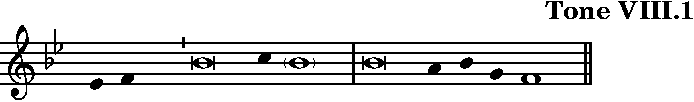
\includegraphics[width=\linewidth]{psalms/psalm91-crop.pdf}

\begin{enumerate}[
    leftmargin=*,
    label=\textsc{ \arabic * }
]
    \item \psalmverse{\textsc{Who-so} dwelleth under the defence of the most Most \textbf{High}:}
        {shall abide under the shadow of \textbf{the} Alm-migh-ty.}

    \item \psalmverse{I will say unto the Lord, `Thou art my refuge and my \textbf{strong}-hold:}
        {my God in \textbf{whom} I will trust'.}

    \item \psalmverse{For he shall deliver thee from the snare of the \textbf{hun}-ter:}
        {and from the \textbf{noi}-some pes-ti-lence.}

    \item \psalmverse{He shall defend thee under his wings, and thou shalt be safe under his \textbf{fea}-thers:}
        {hsi faithfulsness is a \textbf{shield} and buck-ler.}

    \item \psalmverse{Thou shalt not be afraid for any terror by \textbf{night}:}
        {nor for the arrow that \textbf{fli}-eth by day;}

    \item \psalmverse{For the pestilence that walketh in \textbf{dark}-ness:}
        {nor for the sickness that destroyeth \textbf{in} the noon-day.}

    \item \psalmverse{A thousand shall fall beside thée, and ten thousand at thy right \textbf{hand}:}
        {but it shall \textbf{not} come nigh thee.}

    \item \psalmverse{Yea, with thine eyes shalt thou be-\textbf{hold}:}
        {and see the reward of \textbf{the} un-god-ly.}

    \item \psalmverse{Because thou hast said, `The Lord is my \textbf{re}-fuge':}
        {and hast made the Most High thy \textbf{hab}-i-ta-tion,}

    \item \psalmverse{There shall no evil happen unto \textbf{thee}:}
        {neither shall any plague come \textbf{nigh} thy dwelling.}

    \item \psalmverse{For he shall give his angels charge over \textbf{thee}:}
        {to keep \textbf{thee} in all thy ways.}

    \item \psalmverse{They shall bear thee in their \textbf{hands}:}
        {that thou hurt not thy \textbf{foot} a-gainst a stone.}

    \item \psalmverse{Thou shalt go upon the lion and \textbf{ad}-der:}
        {the young lion and the dragon shalt thou tread \textbf{un}-der thy feet.}

    \item \psalmverse{Because he hath set his love upon mé, therefore will I de-\textbf{liv}-er him:}
        {I will set him up, because \textbf{he} hath known my Name.}

    \item \psalmverse{He shall call upon me, and I will \textbf{hear} him:}
        {yea, I am with him in trouble; I will deliver him, and bring \textbf{him} to hon-our.}

    \item \psalmverse{With long life will I satisfy \textbf{him}:}
        {and show him \textbf{my} sal-va-tion.}

    \item[] \psalmverse{Glory be to the Father, and to the \textbf{Son}:}
        {and \textbf{to} the Ho-ly Ghost;}

    \item[] \psalmverse{As it was in the beginning, is now, and ever \textbf{shall} be:}
        {world with-\textbf{out} end. A-men.}
    
\end{enumerate}

\section*{The Short Lesson}

\instruct{Then shall be read one of the following short Lessons, or some other passage of Scripture, at the discretion of the Minister:}

\bibleverse{\textsc{Thou}, O Lord, art in the midst of us, and we are called by thy name. Leave us not, O \textsc{Lord} our God.}
    {Jeremiah 14:9}

\instruct{or}

\bibleverse{\textsc{Come} unto me, all ye that labour and are heavy laden, and I will give you rest. Take my yoke upon you, and learn of me;
for I am meek and lowly in heart: and ye shall find rest unto your souls. For my yoke is easy, and my burden is light.}{Matthew 11:28-30}

\instruct{or}

\bibleverse{\textsc{Now} the God of peace, that brought again from the dead our Lord
Jesus, that great Shepherd of the sheep, through the blood of the
everlasting covenant, make you perfect in every good work to do his
will, working in you that which is well-pleasing in his sight; through
Jesus Christ, to whom be glory for ever and ever. Amen.}{Hebrews 13:20 f.}

\instruct{To which the All respond:}

\begin{tabularx}{\linewidth}{lX}
    \textit{All} & \textbf{Thanks be to God.}
\end{tabularx}

\newpage

\section*{The Brief Responds}

\instruct{The following responsory may be used}

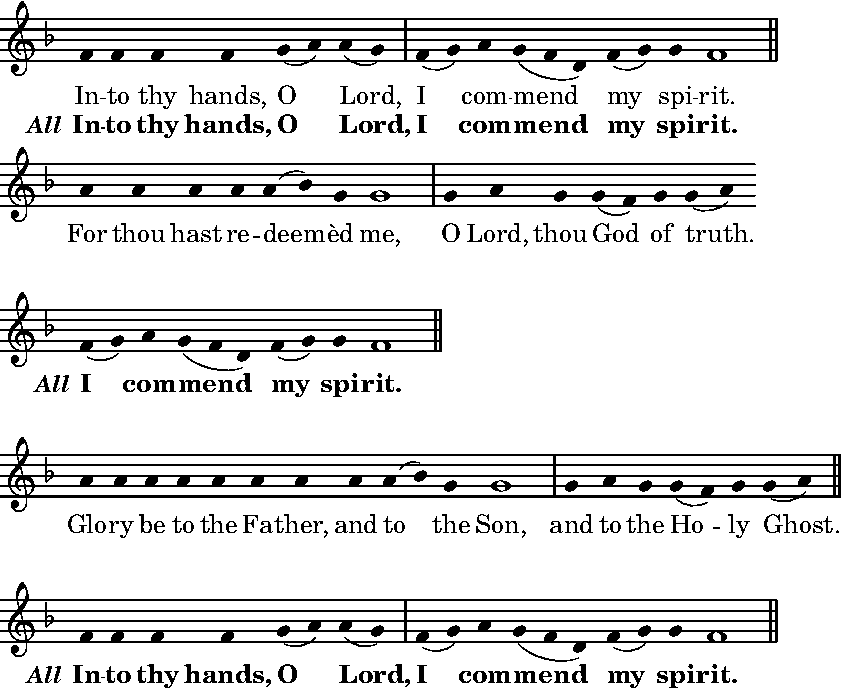
\includegraphics[width=\linewidth]{versicles/inmanustuas-crop.pdf}
\newpage
\section*{The Hymn}

\instruct{This or another hymn may be sung}

\textbf{Te lucis ante terminum}

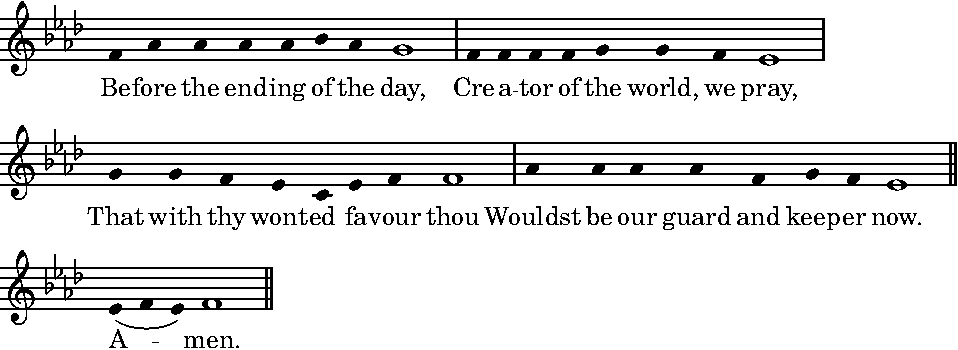
\includegraphics[width=\linewidth]{versicles/telucisanteterminum-crop.pdf}

\begin{prayer}

  From all ill dreams defend our eyes,
  From nightly fears and fantasies;
  Tread underfoot our ghostly foe,
  That no pollution we may know.

  O Father, that we ask be done,
  Through Jesus Christ, thine only son;
  Who, with the Holy Ghost and thee,
  Doth live and reign eternally. Amen.

\end{prayer}

\instruct{Then is sung:}

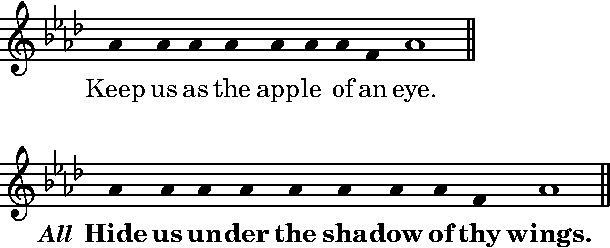
\includegraphics[width=0.7\linewidth]{versicles/appleofaneye-crop.pdf}

\newpage 

\section*{Nunc dimittis}

\textbf{Antiphon}

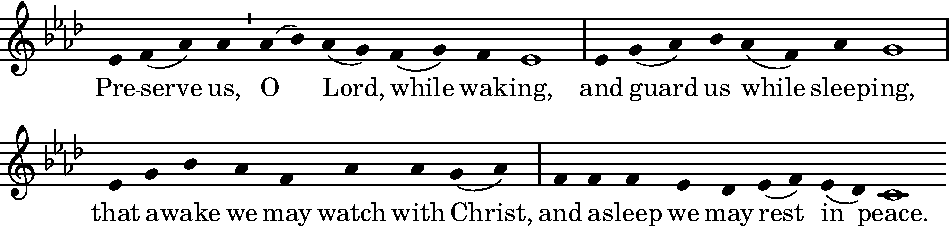
\includegraphics[width=\linewidth]{versicles/nunc-crop.pdf}

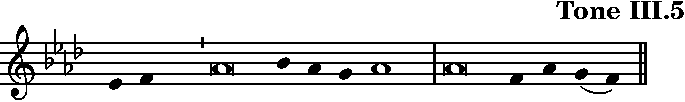
\includegraphics[width=\linewidth]{psalms/psalm31-crop.pdf}

\begin{enumerate}[
    leftmargin=*,
    label=\textsc{\arabic *}
]
    \item \psalmverse{\textsc{Lord, now} lettest thou thy ser-\textbf{vant} de-part ïn peace:}
        {according \textbf{to} thy wörd.}

    \item \psalmverse{\textsc{For mine} eyes have seen \textbf{thy} sal-vä-tion:}
        {which thou hast preparèd before the face of \textbf{all} peo-plë;}

    \item \psalmverse{\textsc{To be} a light to light-\textbf{en} the Gën-tiles:}
        {and to be the glory of thy peo-\textbf{ple} Is-ra-ël.}

    \item[] \psalmverse{\textsc{Glo-ry} be to the Father, \textbf{and} to thë Son:}
        {and to \textbf{the} Ho-ly Ghöst.}

    \item[] \psalmverse{\textsc{As it was} in the beginning, is now, and \textbf{ev}-er shäll be:}
        {world without \textbf{end}. A-mën.}
\end{enumerate}

\textit{Repeat preserve us.}

\newpage

\instruct{During Eastertide, the time between Easter Sunday and Pentecost,
the following form is said:}

\textbf{Antiphon}

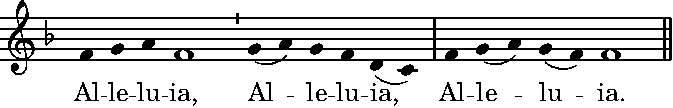
\includegraphics[width=0.9\textwidth]{versicles/easternunc-antiphon-crop.pdf}

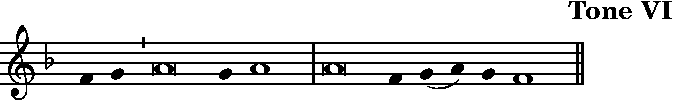
\includegraphics[width=\textwidth]{versicles/easternunc-crop.pdf}

\begin{enumerate}[
    leftmargin=*,
    label=\textsc{\arabic *}
]
    \item \psalmverse{\textsc{Lord, now} lettest thou thy servant depart \textbf{in} peace:}
        {accord-\textbf{ing} tö thy wörd.}

    \item \psalmverse{\textsc{For mine} eyes have seen thy sal-\textbf{va}-tion:}
        {which thou hast preparèd before the face \textbf{of} all peo-ple;}

    \item \psalmverse{\textsc{To be} a light to lighten the \textbf{Gen}-tiles:}
        {and to be the glory of thy \textbf{peo}-plë Is-ra-el.}

    \item[] \psalmverse{\textsc{Glo-ry} be to the Father, and to \textbf{the} Son:}
        {and \textbf{to} thë Ho-ly Ghost.}

    \item[] \psalmverse{\textsc{As it was} in the beginning, is now, and ever \textbf{shall} be:}
        {world with-\textbf{end} ënd. A-men.}
\end{enumerate}

\instruct{Repeat the Alleluia.} 

\newpage
\section*{The Apostles' Creed}

\instruct{Then is said, all together:}

\begin{tabularx}{\linewidth}{lX}

    \textit{All} & \textbf{I believe in God the Father Almighty,} \\
    & \textbf{maker of heaven and earth:} \\
    & \\
    & \textbf{And in Jesus Christ his only Son our Lord,} \\
    & \textbf{who was conceived by the Holy Ghost,} \\
    & \textbf{born of the Virgin Mary,} \\
    & \textbf{suffered under Pontius Pilate,} \\
    & \textbf{was crucified, dead, and buried.} \\
    & \textbf{He descended into hell;} \\
    & \textbf{the third day he rose again from the dead;} \\
    & \textbf{he ascended into heaven,} \\
    & \textbf{and sitteth on the right hand of God the Father Almighty;} \\
    & \textbf{from thence he shall come to judge the quick and the dead.} \\
    & \\
    & \textbf{I believe in the Holy Ghost;} \\
    & \textbf{the holy catholic church;} \\
    & \textbf{the communion of saints;} \\
    & \textbf{the forgiveness of sins;} \\
    & \textbf{the resurrection of the body,} \\
    & \CrossMaltese~\textbf{and the life everlasting.} \\
    & \textbf{Amen.}


\end{tabularx}

\newpage
\section*{The Prayers}

\instruct{After which, all kneel (or whatever is customary), the minister leads:}

\begin{tabularx}{\linewidth}{lX}

    \textit{Minister} & Let us pray. \\
    & \\
    \textit{Minister} & Lord, have mercy upon us. \\
    \textit{All} & \textbf{Christ, have mercy upon us.} \\
    \textit{Minister} & Lord, have mercy upon us. \\
    & \\
    \textit{All} & \textbf{Our Father, who art in heaven,} \\
    & \textbf{hallowed be thy Name;} \\
    & \textbf{thy kingdom come;} \\
    & \textbf{thy will be done;} \\
    & \textbf{on earth as it is in heaven.} \\
    & \textbf{Give us this day our daily bread.} \\
    & \textbf{And forgive our trespasses,} \\
    & \textbf{as we forgive them that trespass against us.} \\
    & \textbf{And lead us not into temptation;} \\
    & \textbf{but deliver us from evil. Amen.} \\

    & \\
    \textit{Minister} & Blessed art thou, Lord God of our fathers: \\
    \textit{All} & \textbf{to be praised and glorified above all for ever.} \\
    & \\
    \textit{Minister} & Let us bless the Father, the Son, and the Holy Ghost: \\
    \textit{All} & \textbf{to praise him and magnify him for ever.} \\
    & \\
    \textit{Minister} & Blessed art thou, O Lord, in the firmament of heaven: \\
    \textit{All} & \textbf{to praised and glorified above all for ever.} \\
    & \\
    \textit{Minister} & The Almighty and mercifful Lord guard us and give us his blessing. \\
    \textit{All} & \textbf{Amen.}

\end{tabularx}

\instruct{A period of silence for reflection on the past day may follow.}
\newpage
\section*{Confession and Prayer for Forgiveness}

\begin{tabularx}{\linewidth}{lX}

    \textit{All} & \textbf{We confess to God Almighty,} \\
    & \textbf{the Father, the Son and the Holy Ghost,} \\
    & \textbf{that we have sinned in thought, word, and deed,} \\
    & \textbf{through our own grievous fault.} \\
    & \textbf{Wherefore we pray God to have mercy upon us.} \\
    & \\
    & \textbf{Almighty God, have mercy upon us,} \\
    & \textbf{forgive us all our sins and deliver us from all evil,} \\
    & \textbf{confirm and strengthen us in all goodness,} \\
    & \textbf{and bring us to life everlasting;} \\
    & \textbf{through Jesus Christ our Lord.} \\
    & \textbf{Amen.}

\end{tabularx}

\instruct{And a priest, if present, may say}

\begin{tabularx}{\linewidth}{lX}
    & May the Almighty and merciful Lord \\
    & grant unto you pardon and remission of all your sins, \\
    & time for amendment of life, \\
    & and the grace and comfort of the Holy Spirit. \\
    \textit{All} & \textbf{Amen.}
\end{tabularx}

\begin{tabularx}{\linewidth}{lX}

    \textit{Minister} & Wilt thou not turn again and quicken us; \\
    \textit{All} & \textbf{that thy people may rejoice in thee.} \\
    & \\
    \textit{Minister} & O Lord, show thy mercy upon us; \\
    \textit{All} & \textbf{and grant us thy salvation.} \\
    & \\
    \textit{Minister} & Vouchsafe, O Lord, to keep us this night without sin; \\
    \textit{All} & \textbf{O Lord, have mercy upon us, have mercy upon us.} \\
    & \\
    \textit{Minister} & O Lord, hear our prayer; \\
    \textit{All} & \textbf{and let our cry come unto thee.}

\end{tabularx}

\section*{Collects}

\instruct{First is said the Collect of the Day, then one or more of the following:}

Visit, we beseech thee, O Lord, this place,
and drive from it all the snares of the enemy;
let thy holy angels dwell herein to preserve us in peace;
and may thy blessing be upon us evermore;
through Jesus Christ our Lord.

\instruct{or}

Lighten our darkness, we beseech thee, O Lord;
and by thy great mercy defend us
from all perils and dangers of this night;
for the love of thy only Son, our Saviour, Jesus Christ.

\instruct{or}

O Lord Jesus Christ, son of the living God,
who at this evening hour didst rest in the sepulchre,
and didst thereby sanctify the grave
to be a bed of hope to thy people:
make us so to abound in sorrow for our sins,
which were the cause of thy passion,
that when our bodies lie in the dust,
our souls may live with thee;
who livest and reignest with the Father and the Holy Ghost,
one God, world without end.

\instruct{or}

Look down, O Lord, from thy heavenly throne,
illuminate the darkness of this night with thy celestial brightness,
and from the sons of light banish the deeds of darkness;
through Jesus Christ our Lord.

\instruct{or}

Be present, O merciful God,
and protect us through the silent hours of this night,
so that we who are wearied
by the changes and chances of this fl eeting world,
may repose upon thy eternal changelessness;
through Jesus Christ our Lord.

\section*{Conclusion}

\begin{tabularx}{\linewidth}{lX}
 
    \textit{Minister} & We will lay us down in peace and take our rest. \\
    \textit{All} & \textbf{For it is thou, Lord, only that makest us dwell in safety.} \\
    & \\
    \textit{Minister} & The Lord be with you; \\
    \textit{All} & \textbf{and with thy spirit.} \\
    & \\
    \textit{Minister} & Let us bless the Lord. \\
    \textit{All} & \textbf{Thanks be to God.} \\
    & \\
    \textit{Minister} & The Almighty and merciful Lord, \\
    & the Father, the Son, and the Holy Ghost, \\
    & bless us and preserve us. \\
    & \\
    \textit{All} & \textbf{Amen.}
 
\end{tabularx}

\section*{Marian Antiphons}

\subsection*{Alma Redemptoris Mater}

\instruct{From Vespers of the Saturday vefore I Sunday in Advent, through II Vespers of the Purification; or if this feast be transferred, through Vespers on Feb. 2nd.}

\textsc{Kindly} Mother of our Redeemer; great portal of heaven ever open, the sea's far-shining star: O succour thy people,
who though fallen strive to rise again. O thou who hast brought forth, to all nature's wonder, nature's Lord, thine own Creator:
Mother yet a Virgin ever more, who at Gabriel's speaking dist receive the Ave: towards us
sinners shew thy pity.

\instruct{From Vespers of Saturday before I Sunday in Advent to None on Vigil of Christmas}

\begin{tabularx}{\linewidth}{lX}
    \textit{Minister} & The Angel of Lord brought tidings unto Mary. \\
    \textit{All} & \textbf{And she conceived by the Holy Ghost.} \\
    \textit{Minister} & Let us pray. \\
    & \\
    & We beseeech thee, O Lord, pour thy grace into our hearts; that, as we have known
the incarnation of thy Son, Jesus Christ, by the message of an angel; so by his
Cross and passion we may be brought unto the glory of his resurrection. Through
the same Christ our Lord. \\
    \textit{All} & \textbf{Amen.} \\
    & \\
    \textit{Minister} & May help divine \CrossMaltese~be with us all, for ever abiding. \\
    \textit{All} & \textbf{Amen.}
\end{tabularx}

\instruct{From I Vespers of Christmas through Vespers on 2nd Feb.}

\begin{tabularx}{\linewidth}{lX}
    \textit{Minister} & After child-bearing thou remainedst a pure Virgin. \\
    \textit{All} & \textbf{Mother of God, intercede for us.} \\
    \textit{Minister} & Let us pray. \\
    & \\
    & O God, who by the child-bearing of a pure Virgin hast bestowed upon all 
    mankind the rewards of everlasting life: grant, we beseech thee; that we may know 
    the succour of her intercession, through whom we have been found worthy to 
    receive the Author of Life, even Jesus Christ thy Son our Lord.\\
    \textit{All} & \textbf{Amen.} \\
    & \\
    \textit{Minister} & May help divine \CrossMaltese~be with us all, for ever abiding. \\
    \textit{All} & \textbf{Amen.}
\end{tabularx}

\subsection*{Ave, Regina caelorum}

\instruct{After the Purification, or Feb. 2nd, to Compline of Wednesday in Holy Week.}

\textsc{Hail}, O Queen, on high enthroned,
Hail, O Lady, by Angels owned:
Jesse's Rod: yea, heaven's portal;
Whence hath shone earth's Light immortal:
Hail, O Virgin, most renowned,
For thy grace and beauty crowned:
Hail, O truly worthy Maiden:
Pray Christ for us so burden-laden.

\begin{tabularx}{\linewidth}{lX}
    \textit{Minister} & May praise by thee accepted be, O hallowed Virgin. \\
    \textit{All} & \textbf{Obtain for me strength against mine enemies.} \\
    \textit{Minister} & Let us pray. \\
    & \\
    & We beseech thee, O Lord, mercifully to assist our infirmity: that like as we do
    now commemorate the blessed Mary Ever-Virgin, Mother of God; so by the help of 
    her intercession we may die to our former sins and rise again to newness 
    of life. Through the same Christ our Lord.
    \\
    \textit{All} & \textbf{Amen.} \\
    & \\
    \textit{Minister} & May help divine \CrossMaltese~be with us all, for ever abiding. \\
    \textit{All} & \textbf{Amen.}
\end{tabularx}

\subsection*{Regina caeli laetare}

\instruct{From Compline of Holy Saturday to None of Saturday in Octave of Pentecost.}

\textsc{Rejoice}, Queen Mother of heaven, alleluia;
Christ whom meetly thou barest is risen, alleluia;
His forsaeying thus fulfilling, alleluia;
Offer to God thy praying, alleluia.

\begin{tabularx}{\linewidth}{lX}
    \textit{Minister} & Rejoice and be exceeding glad, O Virgin Mary, alleluia. \\
    \textit{All} & \textbf{For the Lord is risen indeed, alleluia.} \\
    \textit{Minister} & Let us pray. \\
    & \\
    & O God, who by the resurrection of thy Son our Lord Jesus Christ hast given joy unto the world:
    grant, we beseech thee; that through his Mother, the Virgin Mary, we may obtain the joys of everlasting
    life. Through the same Christ our Lord.
    \\
    \textit{All} & \textbf{Amen.} \\
    & \\
    \textit{Minister} & May help divine \CrossMaltese~be with us all, for ever abiding. \\
    \textit{All} & \textbf{Amen.}
\end{tabularx}

\subsection*{Salve, Regina}

\instruct{From I Vespers of Feast of Trinity, to I Sunday of Advent}

\textsc{All} Hail, O holy Queen, Mother exceeding merciful; Life's spring,
sweet comfort, our Hope-bearer, all hail. To thee our plaint we lift,
children of Eve yet in exile. To thee our aspiring, our longing, and 
weeping, lift we from this vale of sorrow. Ah then, Mary, be our intercessor;
hither vouchsafe to turn thine eyes compassionate, and look upon. And Jesus,
blessed offspring of thy womb, O mother, shew thou to us when earthly
exile endeth. O gentle, O loving, O gracious Virgin Mary.

\begin{tabularx}{\linewidth}{lX}
    \textit{Minister} & Pray for us, O holy Mother of God. \\
    \textit{All} & \textbf{That we may be worthy of the promises of Christ.} \\
    \textit{Minister} & Let us pray. \\
    & \\
    & Almighty, everlasting God, who by the co-operation of the Holy Ghost didst
    prepare the body and soul of the gracious Virgin-Mother Mary to become a dwelling-place
    meet for thy Son: grant that as we rejoice in her commemoration; so by her fervent intercession, we may 
    be delivered from persent evils and from everlasting death. Through the same
    Christ our Lord.
    \\
    \textit{All} & \textbf{Amen.} \\
    & \\
    \textit{Minister} & May help divine \CrossMaltese~be with us all, for ever abiding. \\
    \textit{All} & \textbf{Amen.}
\end{tabularx}

\end{document}
